
\section{Asymptote}
\subsection{Brief description}
\href{http://asymptote.sourceforge.net/}{Asymptote} is "a powerful descriptive vector graphics language that provides a natural coordinate-based framework for technical drawing." In other words, it is a compiled language that generates .eps or .pdf representing any 2D or 3D scene parametrized mathematically. Its hybrid syntax borrows from Python, C and Latex, which can be a bit bewildering at first. Raw asymptote code is customarily stored in the form of a .asy file, which can be edited using the text editor of your choice.
The installation procedure depends on the platform you are using:
\begin{itemize}
\item MacOS X: Asymptote is already shipped with MacTex, so there is nothing to do besides retrieving the Latex distribution
\item Windows: Download the latest executable file from \href{https://sourceforge.net/projects/asymptote/files/}{the official Asymptote page}. Make sure to have a running Latex distribution before attempting to run Asymptote!
\item Linux: Similarly to MacOS X, Asymptote is shipped with the TexLive distribution.
\end{itemize} 
Asymptote files can be compiled directly from a Unix terminal. Simply type \textit{asy myfile.asy} to compile the file and generate the output which by default will be named \textit{myfile.pdf} or \textit{myfile.eps}. The output format can be set using the \textit{settings.outformat="pdf";} instruction in the asy file. On Windows, compilation can be taken care of by TexMaker.
\subsection{Examples}
Two Asymptote output files are presented below, to demonstrate the 2D and 3D capabilities of the language. These examples can be found \href{https://drive.google.com/open?id=0Bzf79yzZcPJJczg3RVhiRFVablk}{here}. Figure \ref{fig:flyby} represents a planetary flyby where the input angles are prescribed to their real value. The trajectory that is displayed is a conic (an hyperbola in this case) which corresponds to the true Keplerian orbit expected in this case.
\begin{figure}[H]
\centering
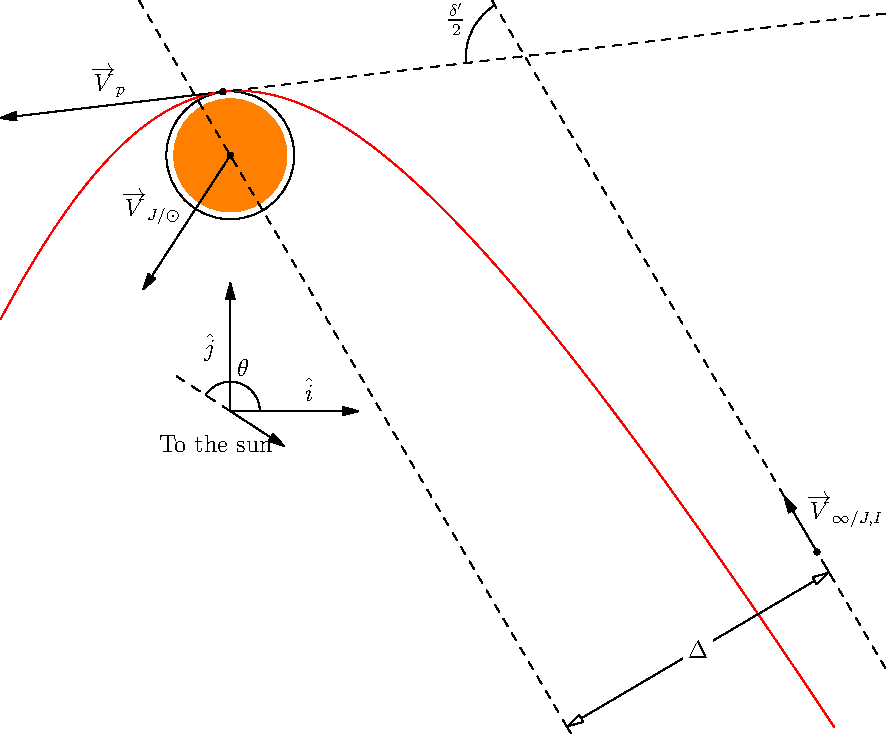
\includegraphics[scale=0.6]{flyby.pdf}
\caption{Planetary flyby (2D scene)}
\label{fig:flyby}
\end{figure}
The example shown on Figure \ref{fig:ECI_to_body} is another illustration of Asymptote capabilities. Here, the body frame of a spacecraft is represented relative to an inertial frame. The spacecraft attitude is parametrized in terms of a set of 321 Euler angles (yaw, pitch, roll) that the user can edit. Recompiling the .asy file for a new attitude will generate the same scene with a different orientation, without requiring the user to edit manually the location of every single satellite feature.
\begin{figure}
\centering
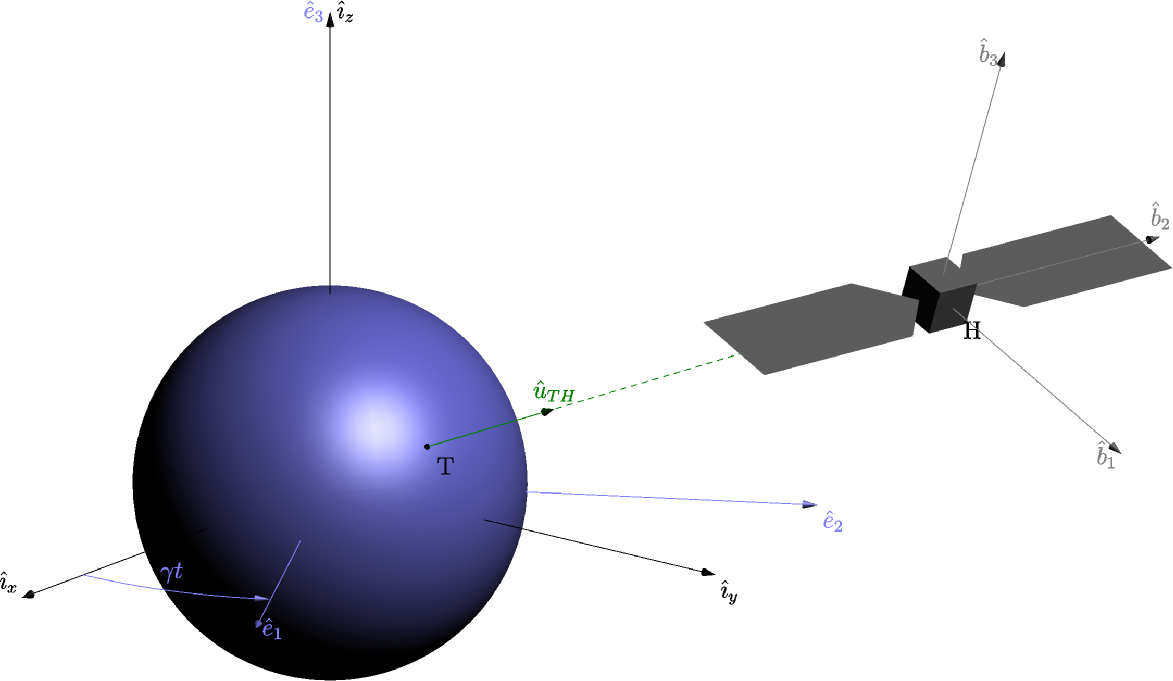
\includegraphics[scale=0.5]{ECI_to_body.pdf}
\caption{Satellite body-frame to inertial frame (3D scene)}
\label{fig:ECI_to_body}
\end{figure}
\subsection{More examples}
The best compilation of examples I have found to date is probably \href{https://drive.google.com/file/d/0Bzf79yzZcPJJc0dWTHNZMkhqTGc/view?usp=sharing}{this one for 2D examples} and
\href{https://drive.google.com/file/d/0Bzf79yzZcPJJYld2cnhqWXZNU28/view?usp=sharing}{ this one for 3D examples}. As the reader will soon notice, these resources are unfortunately not in English. This being said, they are quite self explanatory due to the ubiquitous use of English in the Asymptote language in addition to the (almost) comprehensive list of Asymptote routines they provide. English documentation files, quite comprehensive but maybe less exhaustive can also be found \href{http://asymptote.sourceforge.net/asymptote.pdf}{here} and another one \href{https://math.uchicago.edu/~cstaats/Charles_Staats_III/Notes_and_papers_files/asymptote_tutorial.pdf}{here}.
